\section{Appendix}

\subsection{Mathematica Code: Matching}
The code included in the subsection ``Mathematica Code: Matching'' provides the
Mathematica code that was used to generate the ideal match. Note that this ideal
match was not always used. In the case of the high-gain amplifier it was chosen
to reduce the gain from the maximum gain by almost as much as was possible
($\approx \SI{1}{\deci\bel}$) to ensure the lowest noise figure as was possible.
However, the results given, here, in the code, are for those of an ideal match.
To be clear, a table is provided at the end of the section that enumerates which
length of stub must be used and what length of line (after the stub) must be
used. The length of line between the load and the stub is immaterial since the
line is matched to the load such that $Z_{in} = Z_l = Z_0$, (where $Z_0$ is the
characteristic impedance of the transmission line).

% High Gain Amplifier Mathematica
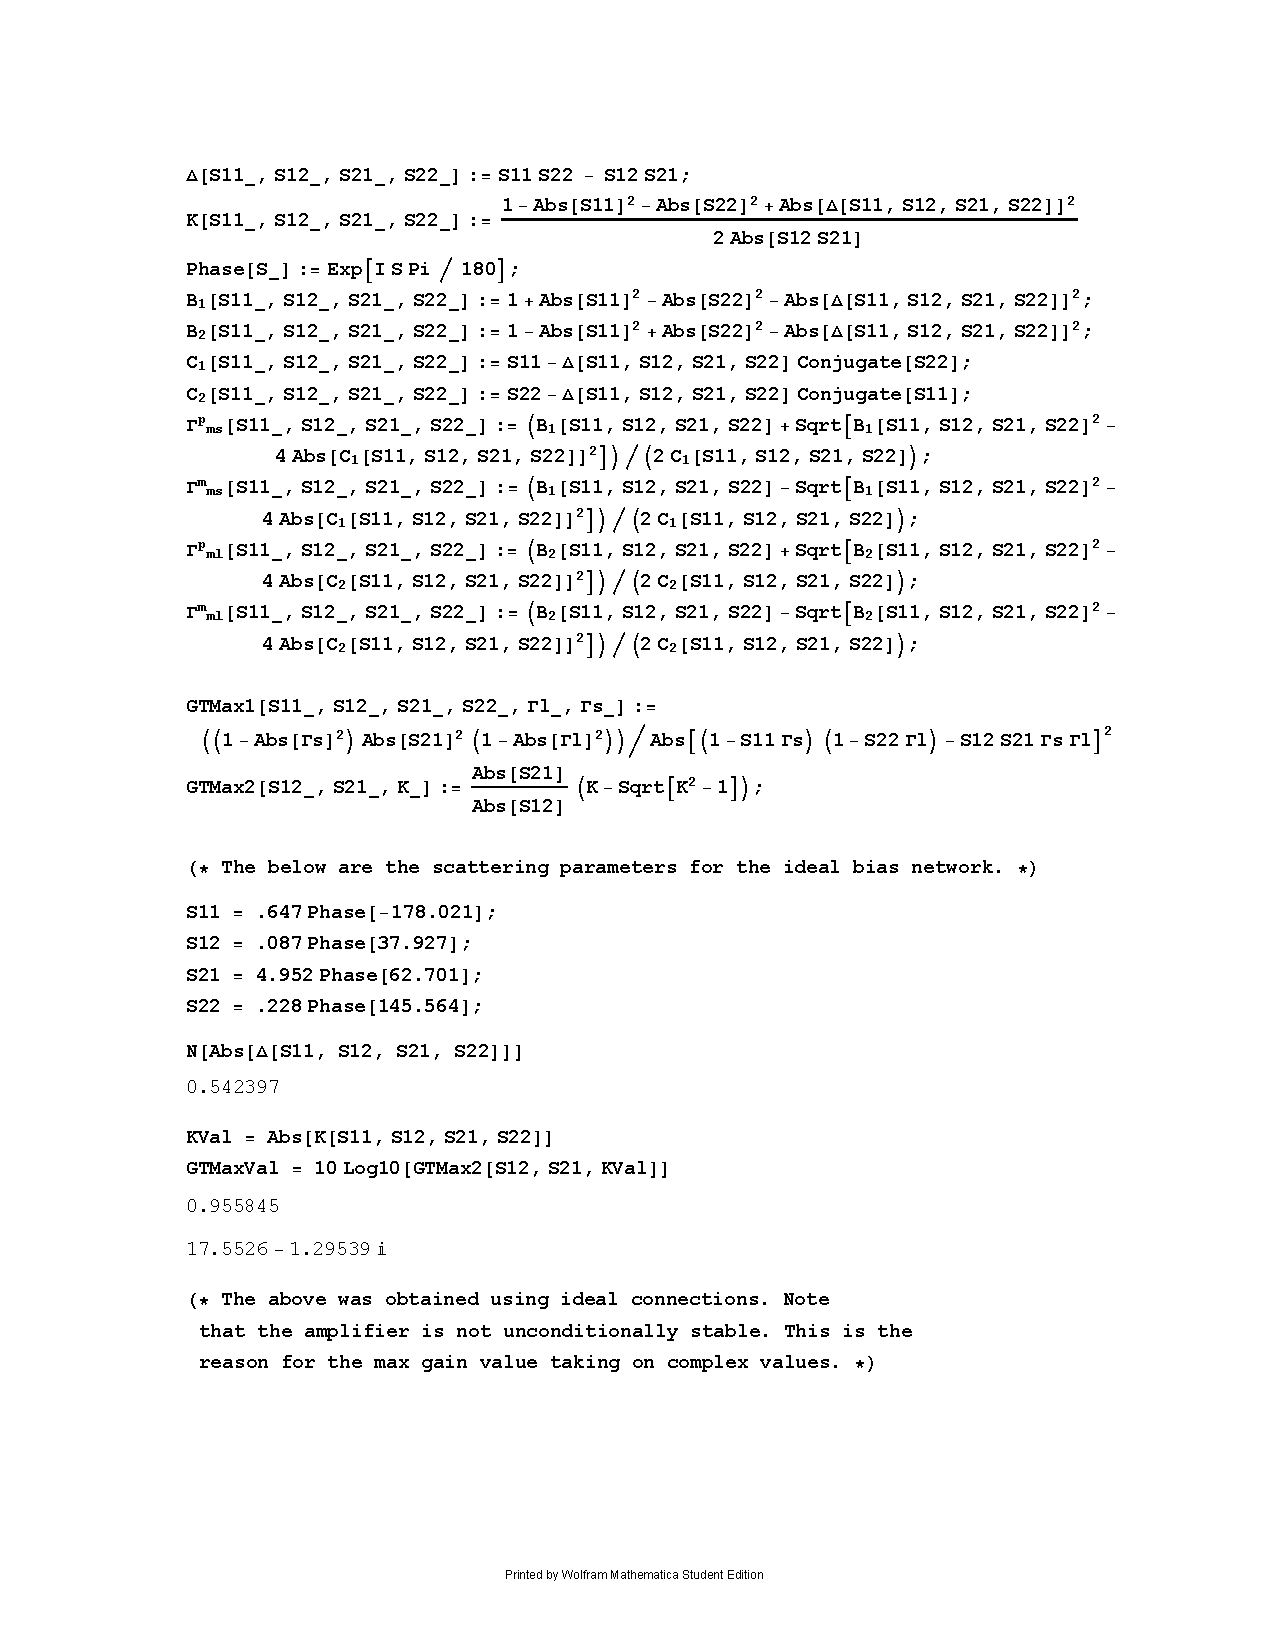
\includepdf[scale=.8,pages=1,clip,trim=0cm 3cm 0cm
2cm,pagecommand=\subsubsection{High Gain Amplifier}]{../res/DesignA2P1Mathematica.pdf}
\includepdf[scale=.8,pages=2-,clip,trim=0cm 3cm 0cm
2cm,pagecommand={}]{../res/DesignA2P1Mathematica.pdf}

\begin{tabular}{|c|c|c|c|}
    \hline & Optimum Reflection Coefficient & Stub Length (\degree) & Series
    Line length (\degree) \\
    \hline Load & .551 \phase{-134.1 \degree} & 52.8 & 5.3 \\
    \hline Source & .811 \phase{162.0 \degree} & 70.2 & 26.9 \\ \hline
\end{tabular}

% Low Noise Amplifier Mathematica
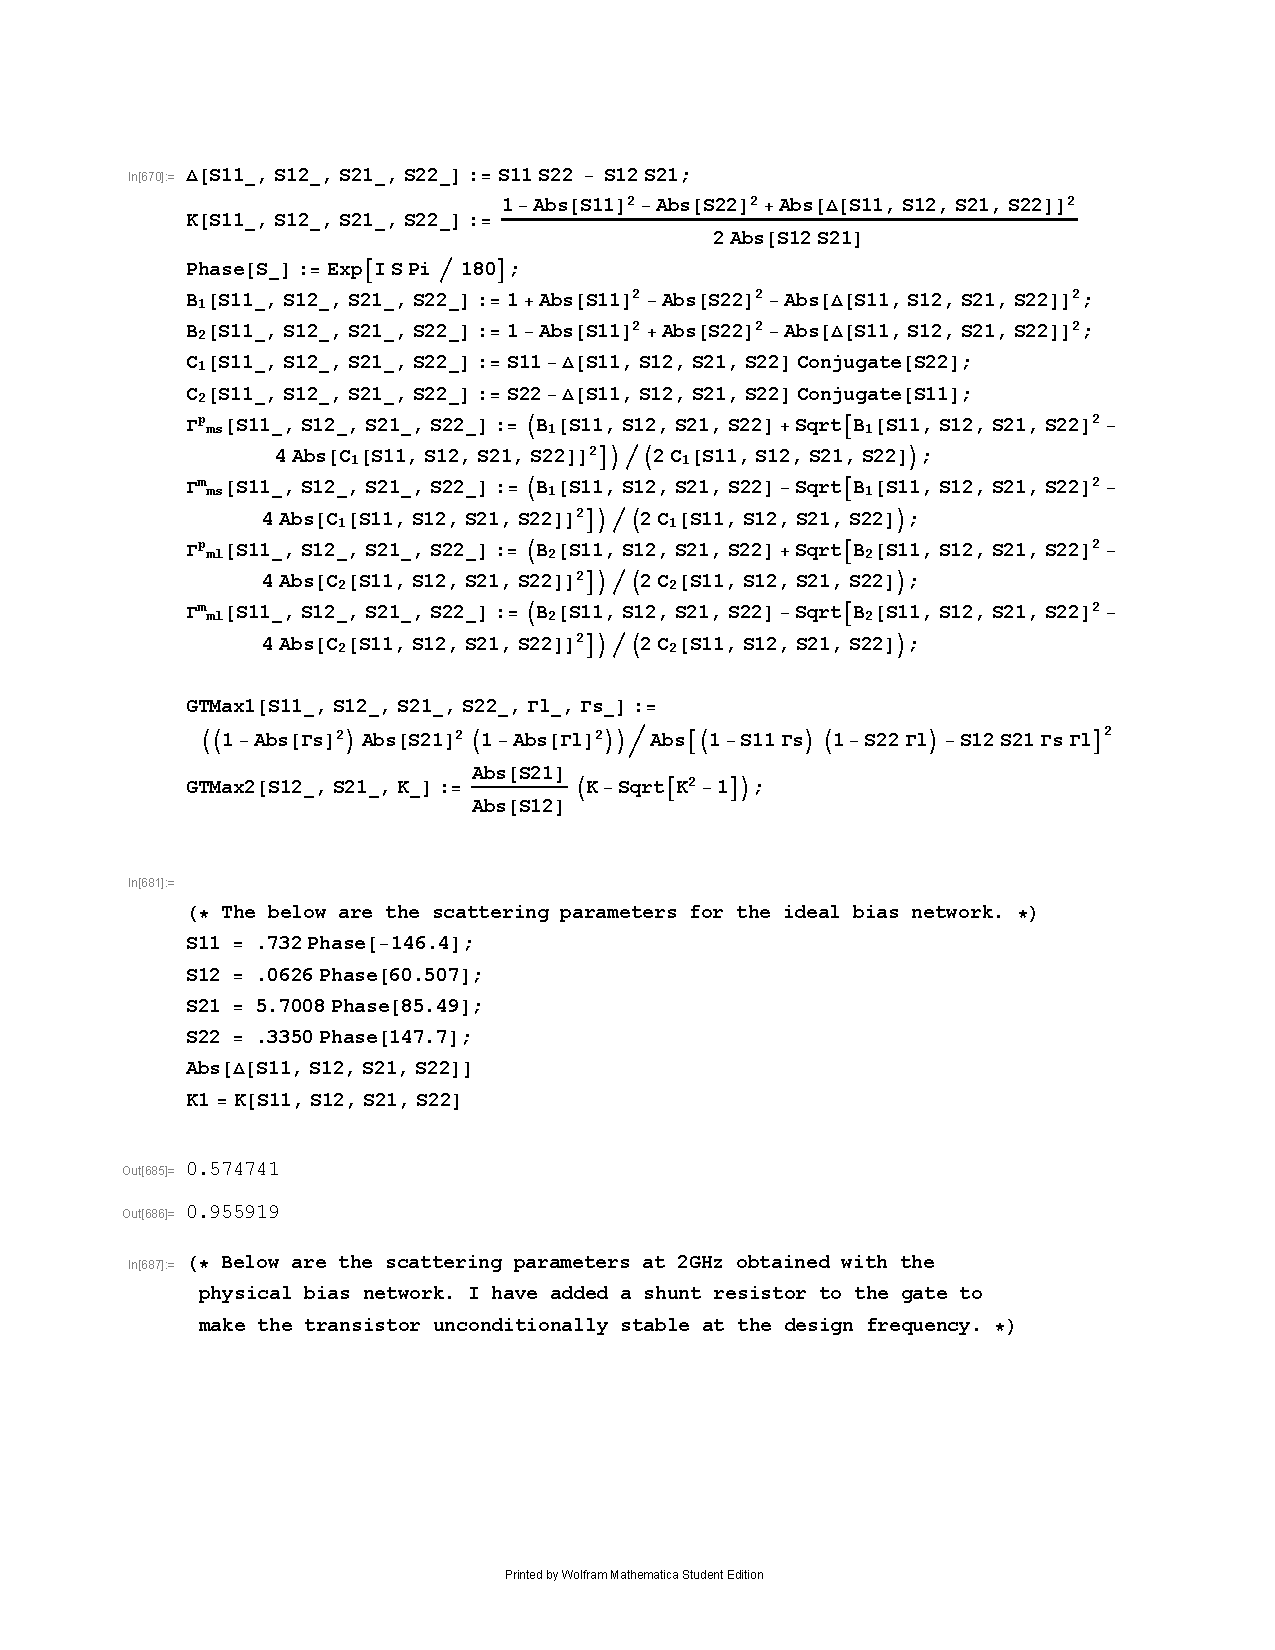
\includepdf[scale=.8,pages=1,clip,trim=0cm 3cm 0cm
2cm,pagecommand=\subsubsection{Low Noise Amplifier}]{../res/DesignA2P2Mathematica.pdf}

\includepdf[scale=.8,pages=2-,clip,trim=0cm 3cm 0cm
2cm]{../res/DesignA2P2Mathematica.pdf}

\begin{tabular}{|c|c|c|c|}
    \hline & Optimum Reflection Coefficient & Stub Length (\degree) & Series
    Line length (\degree) \\
    \hline Load & .998 \phase{-178.1 \degree} & 88 & 181 \\
    \hline Source & .811 \phase{162.0 \degree} & 51.3  & 101 \\ \hline
\end{tabular}

\subsection{MATLAB Scattering Parameter Analysis}

The scattering parameter analysis was really interesting. Unfortunately, I do
not have as much time as I would like to get into the details of the analysis.
Essentially, though, the DC sources can be treated as shorts over the entire
bandwidth of consideration (since DC sources provide no AC voltage/current it
can be shown that, by superposition, they are shorts at AC). This puts the
coupling transmission lines to the ground at AC and, since the source is
grounded, it puts the transmission line sections in parallel with the
transistor. If there was a shunt resistor at the output of the transistor it was
also in parallel with the drain-source transmission line. The series resistor
and the two ``DC block`` capacitors were in series with the two port network.

Thus, the problem can be treated as simply as converting the scattering
parameters of the amplifier into Y parameters and adding the Y parameters of the
transmission lines (and possible the shunt resistor) to the Y parameters of the
transmission line in the following manner:

\[ 
    Y_{int}^{\text{transistor + external elements}} = \begin{pmatrix}
        Y_{11}^{\text{transistor}} + Y^{\text{input transmission line}} &
        Y_{12}^{\text{transistor}} \\
        Y_{21}^{\text{transistor}} & Y_{11}^{\text{transistor}} +
        Y_{22}^{\text{output transmission line ( + shunt resistor)}}
    \end{pmatrix} 
\]

Then, adding on the series stabilizing resistors and the capacitors I can add
the Z parameters of the external resistors and capacitors to the ``new'' 2-port
network once I convert the $Y_{int}$ parameters to their $Z_{int}$ parameters.

:

\[ 
    Z_{final}^{\text{transistor + external elements}} = \begin{pmatrix}
        Z_{11}^{\text{int}} + Z^{\text{input capacitor + series resistor}} &
        Z_{12}^{\text{transistor}} \\
        Z_{21}^{\text{transistor}} & Z_{11}^{\text{int}} +
        Z_{22}^{\text{output capacitor}}
    \end{pmatrix} 
\]

These are the final 2 port parameters that can be converted back to $S_{final}$
scattering parameters. Thus, the chain of conversions goes something like $S
\rightarrow Y \rightarrow Z \rightarrow S$.

% MATLAB High Gain Amplifier below
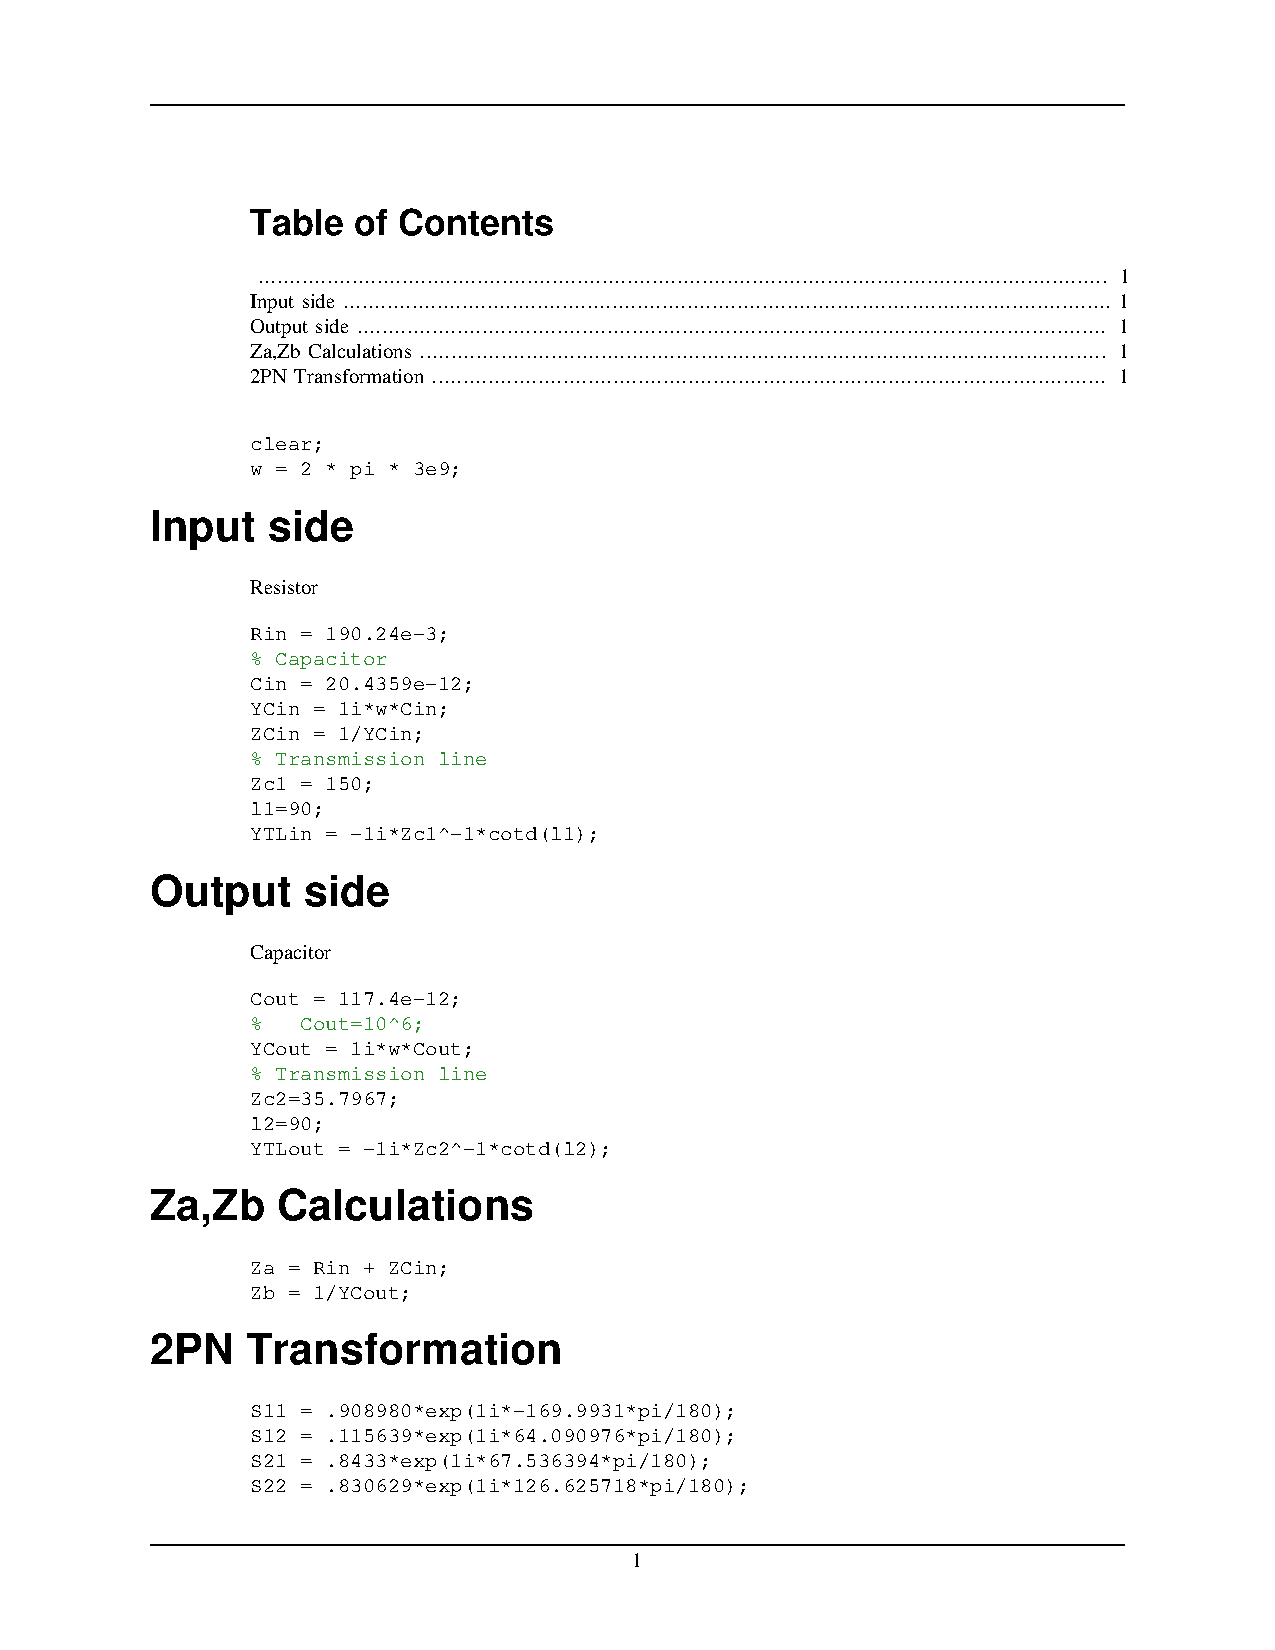
\includepdf[scale=.8,pages=1,clip,trim=0cm 2cm 0cm
0cm,pagecommand=\subsubsection{High Gain Amplifier}]{../res/DesignA2P1.pdf} 

\includepdf[scale=.8,pages=2-,clip,trim=0cm 2cm 0cm
0cm,pagecommand={}]{../res/DesignA2P1.pdf} 

% MATLAB LNA below
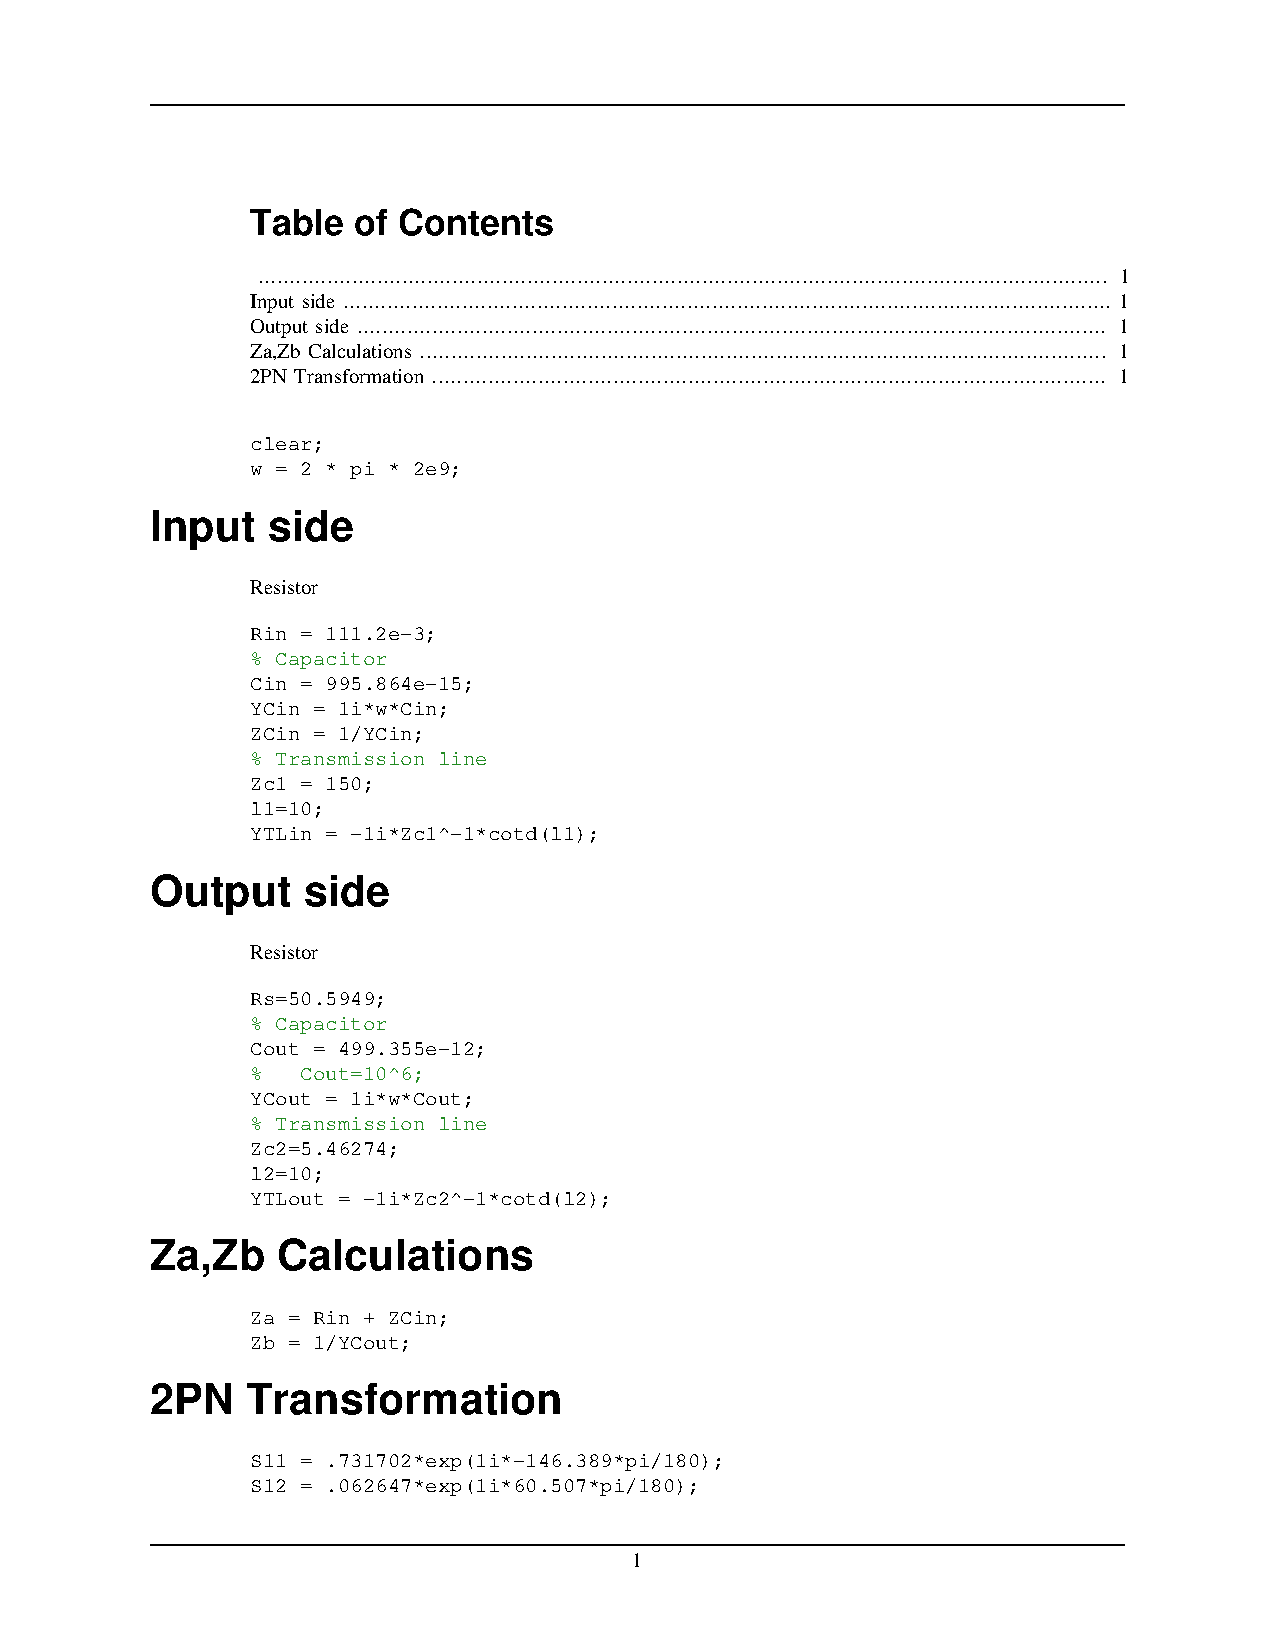
\includepdf[scale=.8,pages=1,clip,trim=0cm 2cm 0cm
0cm,pagecommand=\subsubsection{Low Noise Amplifier}]{../res/DesignA2P2.pdf}

\includepdf[scale=.8,pages=2-,clip,trim=0cm 2cm 0cm
0cm,pagecommand={}]{../res/DesignA2P2.pdf}
